%%%%%%%%%%%%%%%%%%%%%%% file template.tex %%%%%%%%%%%%%%%%%%%%%%%%%
%
% This is a general template file for the LaTeX package SVJour3
% for Springer journals.          Springer Heidelberg 2010/09/16
%
% Copy it to a new file with a new name and use it as the basis
% for your article. Delete % signs as needed.
%
% This template includes a few options for different layouts and
% content for various journals. Please consult a previous issue of
% your journal as needed.
%
%%%%%%%%%%%%%%%%%%%%%%%%%%%%%%%%%%%%%%%%%%%%%%%%%%%%%%%%%%%%%%%%%%%
%
% First comes an example EPS file -- just ignore it and
% proceed on the \documentclass line
% your LaTeX will extract the file if required
\begin{filecontents*}{example.eps}
%!PS-Adobe-3.0 EPSF-3.0
%%BoundingBox: 19 19 221 221
%%CreationDate: Mon Sep 29 1997
%%Creator: programmed by hand (JK)
%%EndComments
gsave
newpath
  20 20 moveto
  20 220 lineto
  220 220 lineto
  220 20 lineto
closepath
2 setlinewidth
gsave
  .4 setgray fill
grestore
stroke
grestore
\end{filecontents*}
%
\RequirePackage{fix-cm}
%
%\documentclass{svjour3}                     % onecolumn (standard format)
%\documentclass[smallcondensed]{svjour3}     % onecolumn (ditto)
%\documentclass[smallextended]{svjour3}       % onecolumn (second format)
\documentclass[twocolumn]{svjour3}          % twocolumn
%
\smartqed  % flush right qed marks, e.g. at end of proof
%
\usepackage{amsmath,graphicx}
\usepackage{import}
\usepackage[ruled]{algorithm2e}
%
% \usepackage{mathptmx}      % use Times fonts if available on your TeX system
%
% insert here the call for the packages your document requires
%\usepackage{latexsym}
% etc.
%
% please place your own definitions here and don't use \def but
% \newcommand{}{}
%
% Insert the name of "your journal" with
% \journalname{myjournal}
%
\begin{document}

\title{Low-complexity, Sub-band DPD with Sequential Learning%\thanks{Grants or other notes
%about the article that should go on the front page should be
%placed here. General acknowledgments should be placed at the end of the article.}
}
\subtitle{Novel Algorithms and \textsc{Warp}Lab Implementation}

%\titlerunning{Short form of title}        % if too long for running head

\author{Chance Tarver         \and
        Mahmoud Abdelaziz \and
        Lauri Anttila \and
        Mikko Valkama \and
        Joseph~R.~Cavallaro
}

%\authorrunning{Short form of author list} % if too long for running head

\institute{Chance Tarver and Joseph R. Cavallaro \at
	Department of Electrical and Computer Engineering\\
	Rice University, Houston, TX, 77005, USA\\
	\email{\{cat12,cavallar\}@rice.edu}           %  \\
	%             \emph{Present address:} of F. Author  %  if needed
	\and
	Mahmoud Abdelaziz, Lauri Anttila and Mikko Valkama \at
	Department of Electronics and Communication Engineering\\
	Tampere University of Technology, Finland
}


\date{Received: date / Accepted: date}
% The correct dates will be entered by the editor

\maketitle

%Need to revise to include update.
%Current number of words: 138. 
%Recommended: 150 to 250 word
\begin{abstract}
Digital predistortion (DPD) is an effective way of mitigating spurious emission violations without the need of a significant power reduction in the transmitter, thus providing better power efficiency and network coverage. 
In this paper an iterative version of the IM3 sub-band DPD, proposed earlier by the authors, is presented. 
The DPD learning is iterated between the higher and lower IM3 sub-bands until a satisfactory performance is achieved for both of them. 
A sequential DPD learning procedure is also presented in order to reduce the hardware complexity when higher order nonlinearities are incorporated in the DPD learning. 
Improvements on the convergence speed of the adaptive DPD learning are also achieved via incorporating a variable learning rate and training from previous values. 
A \textsc{Warp}Lab implementation of the proposed DPD is also shown with excellent suppression of the targeted spurious emissions. 
\keywords{Adaptive filters \and carrier aggregation \and digital predistortion \and nonlinear distortion \and power amplifier \and software-defined radio \and spectrally-agile radio \and spurious emission. }
% \PACS{PACS code1 \and PACS code2 \and more}
% \subclass{MSC code1 \and MSC code2 \and more}
\end{abstract}

\section{Introduction}
In mobile devices transmitting spectrally aggregated carriers with a single power amplifier (PA), some of the intermodulation distortion (IMD) components created by the nonlinear PA will fall on the spurious region as shown in Fig. \ref{fig:PSD} and may seriously violate the spurious emission limits \cite{Commag_abdelaziz,3GPP_CA_Emissions_1,3GPP_CA_Emissions_2,LaehteensuoMay2013}. 
To satisfy the stringent emission requirements in such scenarios, devices may need to considerably back off their transmit power from the nominal maximum value (e.g., +23 dBm in 3GPP LTE uplink). 
However, reducing the transmit power in order to fulfill the emission mask will necessarily reduce the uplink coverage. 
An alternative solution to power back-off is to use digital predistortion (DPD) for reducing the unwanted spectral emissions \cite{P.RoblinJan.2008,J.KimJan.2013,S.A.BassamAug.2012,ICASSP2014,Commag_abdelaziz}. 

In \cite{ICASSP2014}, the third-order IMD at the IM3$\pm$ sub-bands were considered separately, while not taking into consideration the mutual effect of each of the IM3 sub-band DPDs over the other. 
An \textsc{fpga} implementation of this solution has also been presented by the authors in \cite{Asilomar2015} demonstrating real-time processing of the adaptive DPD learning solution.
An extension of the DPD solution in \cite{ICASSP2014,Asilomar2015} is proposed in this paper, where an iterative learning algorithm is used between the two IM3 sub-bands until they are both properly suppressed. 
Moreover, in \cite{TMTT_SubbandDPD}, higher nonlinearity orders were introduced in addition to the third-order nonlinearity processing in \cite{ICASSP2014,Asilomar2015}.
A \textsc{Warp}Lab implementation of an iterative version of this higher order sub-band DPD is also presented in this paper with additional ideas added to reduce the complexity and/or improve the learning speed of the proposed DPD. 
In summary, the main novelty of this paper is as follows:
\begin{itemize}
	\item Introducing an iterative version of the previously proposed sub-band DPD. This solution iterates between the different spurious components, such as the IM3+ and IM3-, until a satisfactory performance is achieved for each of them.
	\item The learning of the higher order nonlinearities in each sub-band is done sequentially, one basis function at a time in ascending order. 
	This has the advantage of reducing the hardware complexity by essentially using one learning module for all the nonlinearity orders. 
	An additional flexibility advantage is that we can stop adding higher orders in the learning phase once a sufficient spurious emission suppression is achieved, thus further reducing the complexity.
	\item In order to improve the convergence speed of the proposed solution, two modifications have been introduced in this paper. 
	The first is using a variable learning rate during the DPD coefficient learning to have a fast convergence at the initial phase of the learning while not sacrificing the steady state error. 
	The second modification is that the DPD coefficients are stored once they are converged, and act as a starting point for learning once the same carrier configuration is transmitted again.
	\item A \textsc{Warp}Lab implementation of the proposed solution is done demonstrating effective performance of the proposed solution using real hardware equipment. 
\end{itemize}

This paper is organized as follows. 
In Section II, the modeling of the spurious emissions at the IM3 sub-bands and their mutual effects are presented.
The proposed iterative sub-band DPD processing is also introduced in this section. 
In Section III, sequential learning of the DPD coefficients is proposed to reduce the hardware complexity. 
In Section IV, two methods are proposed for improving the convergence time. 
In Section V, the overall DPD system flow is presented. 
In Section VI, we show the results from testing the proposed algorithms on the \textsc{Warp}Lab platform. 
Finally, in Section VII, we conclude the paper.

\begin{figure}
	\centering
	%\vspace{0.5cm}
	\centerline{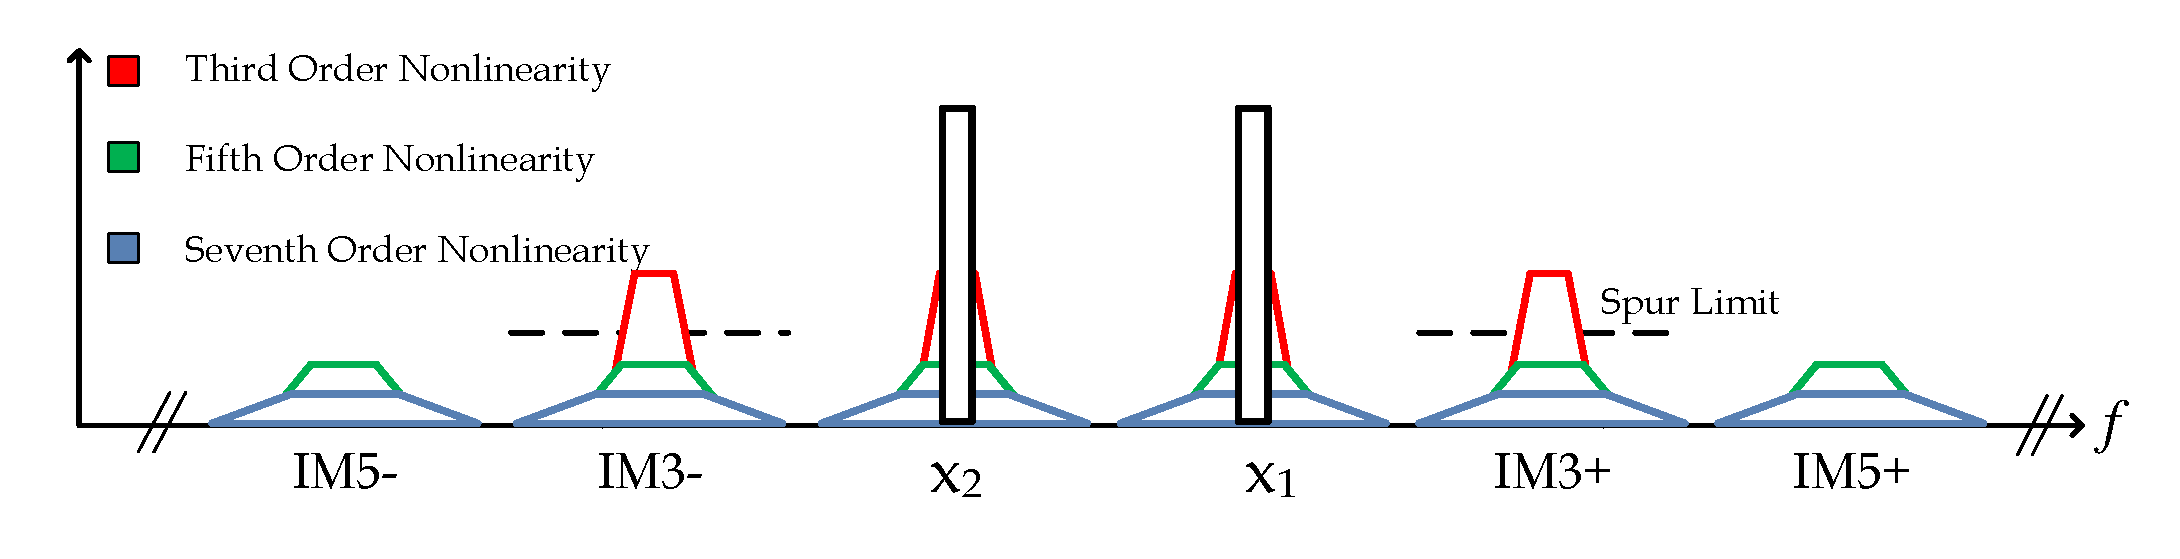
\includegraphics[width=0.4\textwidth]{./Figures/PSD.pdf}}
	\caption[]{Power spectral density of a carrier aggregated signal after being applied through a nonlinear PA.
		Nonlinearity orders up to the seventh are shown, and only IM3$\pm$ spurious emissions are presented as they are the main focus of this work.}
	\label{fig:PSD}
\end{figure}

\section{Spurious Component Modeling and Iterative IM3 Sub-band DPD Processing}
\label{sec:Analysis}
In \cite{ICASSP2014}, a decorrelation-based sub-band DPD was proposed to mitigate the spurious emissions at the IM3$\pm$ sub-bands. 
However, the mutual effect of, for example, the IM3+ sub-band DPD on the IM3- sub-band was not taken into consideration. 
In this work, we propose an iterative sub-band DPD that starts with linearizing the IM3+ sub-band, and then after applying the IM3+ sub-band DPD, the learning is switched to the IM3- sub-band. 
Since each of the IM3$\pm$ sub-band DPDs has an effect on the other sub-band, the proposed DPD iterates the learning between the two sub-bands until both spurious emissions are sufficiently suppressed.

To further illustrate this behavior, a mathematical analysis is introduced in this section to show the impact of the IM3+ sub-band DPD on the IM3- sub-band when a dual carrier signal is applied to a nonlinear PA. 
This analysis will provide a theoretical foundation and motivation for our work. 
For simplicity of the presentation, we restrict our analysis in this section to third-order nonlinearity. 
However, in the actual \textsc{Warp}Lab experiments, higher order nonlinearities are included in the DPD processing.
The analysis is carried out at composite baseband equivalent level, and the two component carriers (CC's) are assumed to be separated by $2 f_{IF}$. Thus, the composite baseband equivalent PA input and output signals, $x(n)$ and $y(n)$, read
\begin{align}
\small
x(n) &= x_1(n) e^{j 2\pi \frac{f_{IF}}{f_s} n} + x_2(n) e^{-j 2\pi \frac{f_{IF}}{f_s} n}, \label{eq:PA_In} \\
y(n) &= \beta_1 x(n) + \beta_3 |x(n)|^2 x(n), \label{eq:PA}
\end{align}
\normalsize 
where $\beta_1$ and $\beta_3$ are unknown PA coefficients, and $x_1(n)$ and $x_2(n)$ are the baseband equivalents of the input CCs. 
Through direct substitution of (\ref{eq:PA_In}) in (\ref{eq:PA}), the baseband equivalent positive and negative IM3 terms read
\begin{align}
y_{IM3_+}(n) &= \beta_3  x_2^*(n)x_1^2(n), \label{eq:IM3_out} \\
y_{IM3_-}(n) &= \beta_3  x_1^*(n)x_2^2(n). 
\label{eq:IM3_neg_out}
\end{align}
\normalsize
The idea proposed in \cite{ICASSP2014}, for suppressing the IMD at the IM3+ sub-band for example, is to inject a proper additional low-power cancellation signal to (\ref{eq:PA_In}), located at three times $f_{IF}$, such that spurious emission at the IM3+ sub-band at the PA output is suppressed. 
Stemming from the signal structure in (\ref{eq:IM3_out}), the injection signal is of the form $x_2^*(n)x_1^2(n)$ but should be scaled properly with a complex DPD coefficient denoted here by $\alpha$. 
Thus, incorporating such DPD processing, the composite baseband equivalent PA input signal now reads
\begin{align}
\small
\tilde{x}(n) &= x_1(n) e^{j 2\pi \frac{f_{IF}}{f_s} n} + x_2(n) e^{-j 2\pi \frac{f_{IF}}{f_s} n} \nonumber\\ 
&+ \alpha(x_2^*(n)x_1^2(n)) e^{j 2\pi \frac{3 f_{IF}}{f_s} n}. \label{eq:PA_In_DPD}
\end{align}
\normalsize
%where $\tilde{x}(n)$ indicates the PA input signal with DPD included. 
Substituting now $\tilde{x}(n)$ in (\ref{eq:PA}), the IM3 components at PA output read
\begin{align}
\small
\tilde{y}_{IM3_+}(n) &= (\beta_3 + \beta_1 \alpha) x_2^*(n) x_1^2(n) \nonumber\\
& \quad + 2 \beta_3 \alpha (|x_1(n)|^2 + |x_2(n)|^2) x_2^*(n) x_1^2(n) \nonumber\\ 
& \quad + \beta_3 |\alpha|^2 \alpha |x_1(n)|^4 |x_2(n)|^2 x_2^*(n) x_1^2(n), \label{eq:IM3_+}\\
\tilde{y}_{IM3_-}(n) &=  \beta_3 x_1^*(n) x_2^2(n) + \boxed{2 \beta_3 \alpha^* |x_1(n)|^2 x_1^*(n) x_2^2(n)}. \label{eq:IM3_-}
\end{align}
\normalsize
It can be seen from (\ref{eq:IM3_+}) and (\ref{eq:IM3_-}) that the spurious emissions at both IM3 sub-bands are dependent on the DPD parameter $\alpha$, despite the cancellation signal being injected only at the IM3+ sub-band. 
In particular, an additional fifth-order term which depends on $\alpha$ appears at the IM3- sub-band, which is shown inside the box in (\ref{eq:IM3_-}). 
Despite the magnitude of this term being quite small, it becomes considerable when the PA exhibits strong nonlinearities. 
This represents the theoretical basis of the mutual effect the IM3+ sub-band DPD has on the two IM3 sub-bands.

In \cite{ICASSP2014}, the learning of the DPD parameter $\alpha$, for the IM3+ sub-band, for example, was formulated to minimize the correlation between the IMD at the considered IM3 sub-band and the distortion basis $x_2^*(n)x_1^2(n)$. 
This correlation minimization will eventually minimize the distortion at the considered sub-band effectively, as demonstrated in \cite{ICASSP2014,Asilomar2015}. 
However, optimizing the DPD parameter $\alpha$ to minimize the power at the IM3+ sub-band, will affect the IM3- sub-band as well, as shown in (\ref{eq:IM3_+}) and (\ref{eq:IM3_-}). 
That is why an iterative sub-band DPD learning is proposed in this paper, in the case both IM3 sub-bands are required to be mitigated effectively. 
First we start by learning the DPD coefficients for the IM3+ sub-band, then after injecting the IM3+ cancellation signal, the emissions at the IM3- sub-band are raised a little above their original levels due to the mutual effect described earlier. 
Then, the DPD learning is switched to the IM3- sub-band, which then also affects the IM3+ sub-band. 
That is why an extra iteration is required at the IM3+ sub-band such that the spurious emissions are reduced at both IM3 sub-bands. This will be demonstrated in the \textsc{Warp}Lab experimental results in Section \ref{sec:WARPLabResults}.

In the following sections, modifications are introduced to the proposed sub-band DPD in order to reduce the complexity, improve the convergence speed, or both. 
These aspects are particularly important for mobile devices, which is the main scope of this work.

\section{Sequential Learning of IM3 sub-band DPD Coefficients}
\label{sec:Sequential_Learning}
A detailed analysis of the nonlinear distortions at the IM3 sub-band has been done in \cite{TMTT_SubbandDPD} when a ninth-order PA is excited with a dual carrier signal as in (\ref{eq:PA_In}). 
We hereby present the distortion components up to the ninth order at the IM3+ sub-band, which read
\begin{align}
\small
u^+_3(n) &= x_2^*(n)x_1^2(n), \label{eq:IM3_BasisFunctions1}\\
u^+_5(n) &= u^+_3(n) \times (2 |x_1(n)|^2 + 3 |x_2(n)|^2),  \label{eq:IM3_BasisFunctions2}\\
u^+_7(n) &= u^+_3(n) \times (3 |x_1(n)|^4 + 6 |x_2(n)|^4 \nonumber\\
& \quad + 12 |x_1(n)|^2 |x_2(n)|^2) \label{eq:IM3_BasisFunctions3},\\
u^+_9(n) &= u^+_3(n) \times (4 |x_1(n)|^6 + 10|x_2(n)|^6 \nonumber\\
&\quad + 30 |x_1(n)|^4 |x_2(n)|^2 + 40 |x_1(n)|^2 |x_2(n)|^4). \label{eq:IM3_BasisFunctions4}
\end{align}
\normalsize
Similarly, for the IM3- sub-band, the distortions terms $u^-_3(n)$ are simply obtained by interchanging $x_1(n)$ and $x_2(n)$ in (\ref{eq:IM3_BasisFunctions1})-(\ref{eq:IM3_BasisFunctions4}).

The proposed DPD was based on injecting the above basis functions at the IM3+ sub-band with proper scaling such that the distortion at the IM3+ sub-band is minimized. 
The composite baseband equivalent PA input signal with $Q^{th}$ order sub-band DPD processing thus reads 
\begin{align}
\small
\tilde{x}(n) &=  x(n) + \left[\sum_{\substack{q=3 \\ q \text{ odd}}}^{Q} \alpha^+_{q,n} \star  u^+_q(n)\right]e^{j 2\pi \frac{3 f_{IF}}{f_s} n}
\label{eq:PA_In_with_IM3_DPD}
\end{align}
\normalsize

The $q^{th}$ order DPD coefficients $\alpha^+_{q,n}$ are obtained such that the correlation is minimized between the nonlinear distortion observed at the PA output at the IM3+ sub-band, and the nonlinear basis functions in (\ref{eq:IM3_BasisFunctions1})-(\ref{eq:IM3_BasisFunctions4}). 
This is formulated as a simple block-adaptive learning approach, where the following vector based notations are defined
\begin{align}
\small
\boldsymbol{\alpha}^+_q(m) &= [\alpha^+_{q,0}(m)\:\:\alpha^+_{q,1}(m)\:\: ... \:\: \alpha^+_{q,N}(m)]^T, \\
\bar{\boldsymbol{\alpha}}^+(m) &= [\boldsymbol{\alpha}^+_3(m)^T \:\: \boldsymbol{\alpha}^+_5(m)^T \:\: ... \:\: \boldsymbol{\alpha}^+_Q(m)^T]^T, \\
\textbf{u}^+_q(n_m) &= [u^+_q(n_m)\:\:u^+_q(n_m-1) \:\: ... \:\: u^+_q(n_m-N)]^T, \\
\bar{\textbf{u}}^+(n_m) &= [\textbf{u}^+_3(n_m)^T \:\: \textbf{u}^+_5(n_m)^T  \:\: ... \:\: \textbf{u}^+_Q(n_m)^T ]^T, \\
\bar{\textbf{U}}^+(m) &= [\bar{\textbf{u}}^+(n_m) \:\: ... \:\: \bar{\textbf{u}}^+(n_m+M-1)],
\end{align}
\normalsize
where $N$ denotes the DPD filter memory depth, and $n_m$ denotes the first sample of block $m$, with block size $M$.
Consequently, the DPD block-adaptive parameter learning update then reads
\begin{align}
\small
&\textbf{e}^+(m) = [\tilde{y}_{IM3_+}(n_m) \:\: ... \:\: \tilde{y}_{IM3_+}(n_m+M-1)]^T, \\
&\bar{\boldsymbol{\alpha}}^+(m+1) = \bar{\boldsymbol{\alpha}}^+(m) - \mu \: \bar{\textbf{U}}^+(m)\textbf{e}^{+*}(m), 
\label{eq:BlockAdaptive}
\end{align}
\normalsize
where $\tilde{y}_{IM3_+}(n)$ denotes the baseband equivalent observation of the PA output at the IM3+ sub-band with the current DPD coefficients, and $\textbf{e}^{+*}(m)$ refers to the element-wise conjugated error signal vector, while $\bar{\textbf{U}}^+(m)$ denotes the filter input data matrix, all within the processing block $m$. 
The obtained new DPD coefficients $\bar{\boldsymbol{\alpha}}^+(m+1)$ are then applied on the next block of samples, as illustrated in \cite{Asilomar2015}.

In order to reduce the hardware complexity of the DPD, a sequential learning of the DPD coefficients is proposed in this paper instead of learning the DPD coefficients for all the nonlinearity orders concurrently. 
The idea is to first train the DPD for the third-order coefficient, and after injecting the scaled third-order basis function at the target IM3 sub-band, we start training for the fifth-order coefficient using the residual IMD at the target sub-band, and so on. 
This proposed learning algorithm has two advantages. 
The first is that only one hardware module needs to be used for training all the DPD nonlinearity orders thus reducing the hardware overhead due to DPD learning, which is an important aspect especially for small devices. 
The second advantage is that we can stop training the DPD once a sufficient performance is achieved. 
For example, if after doing the third-order training, the transmitter already satisfies the emission limits, then there is no need to train the DPD for higher orders. 
This will save the complexity in both the DPD training phase and in the actual DPD filtering as well.

However, for fast and smooth learning of the proposed sub-band DPD coefficients, a basis function orthogonalization procedure was proposed earlier in \cite{TMTT_SubbandDPD}. 
In this paper, we use an orthogonalization procedure which allows us to learn the DPD coefficients with different orders sequentially instead of concurrently. 
The idea of the orthogonalization and learning procedure in this paper is to first generate the third-order basis function and train the DPD for this basis function. 
Then the projection of the third-order basis function onto the fifth-order basis function is subtracted from the fifth-order basis function in order to obtain the new orthogonalized fifth-order basis function, which is then used to train the DPD for the fifth-order nonlinearity, and so on. 
Once the spurious emissions satisfy the emission regulations, the DPD training is stopped to save further higher-order processing that may not be required, depending on the transmission scenario and TX power level. 
Using the standard vector dot product, the new orthogonalized basis functions $v^\pm_q(n)$ used for DPD learning thus read
\begin{align}
\small
v^\pm_3(n) &= u^\pm_3(n), \label{eq:IM3_OrthBasis_1} \\
v^\pm_5(n) &= u^\pm_5(n) - \frac{dot(u^\pm_5(n),v^\pm_3(n))}{||v^\pm_3(n)||^2} v^\pm_3(n), \label{eq:IM3_OrthBasis_2} \\
v^\pm_7(n) &= u^\pm_7(n)   - \frac{dot(u^\pm_7(n),v^\pm_3(n))}{||v^\pm_3(n)||^2} v^\pm_3(n) \nonumber\\
&\:\:\:\:\:\:\:\:\:\:\:\:\:\:\:\:\:\: - \frac{dot(u^\pm_7(n),v^\pm_5(n))}{||v^\pm_5(n)||^2} v^\pm_5(n), \label{eq:IM3_OrthBasis_3}\\
v^\pm_9(n) &= u^\pm_9(n) - \frac{dot(u^\pm_9(n),v^\pm_3(n))}{||v^\pm_3(n)||^2} v^\pm_3(n) \nonumber\\
&\:\:\:\:\:\:\:\:\:\:\:\:\:\:\:\:\:\: - \frac{dot(u^\pm_9(n),v^\pm_5(n))}{||v^\pm_5(n)||^2} v^\pm_5(n) \nonumber\\ 
&\:\:\:\:\:\:\:\:\:\:\:\:\:\:\:\:\:\:	- \frac{dot(u^\pm_9(n),v^\pm_7(n))}{||v^\pm_7(n)||^2} v^\pm_7(n). \label{eq:IM3_OrthBasis_4}
\end{align}
\normalsize
Despite the reduced complexity that is achieved from the proposed sequential DPD learning, the learning time is now increased compared to the case when we learn all the DPD nonlinearity orders concurrently. 
Two algorithm modifications are thus proposed in the next section for improving the convergence speed of the proposed DPD.

\import{./}{Section_Speedup.tex}

\section{Overall DPD System Flow}
\label{sec:SystemFlow}
\begin{figure*}
	\centering
	%\vspace{0.5cm}
	\centerline{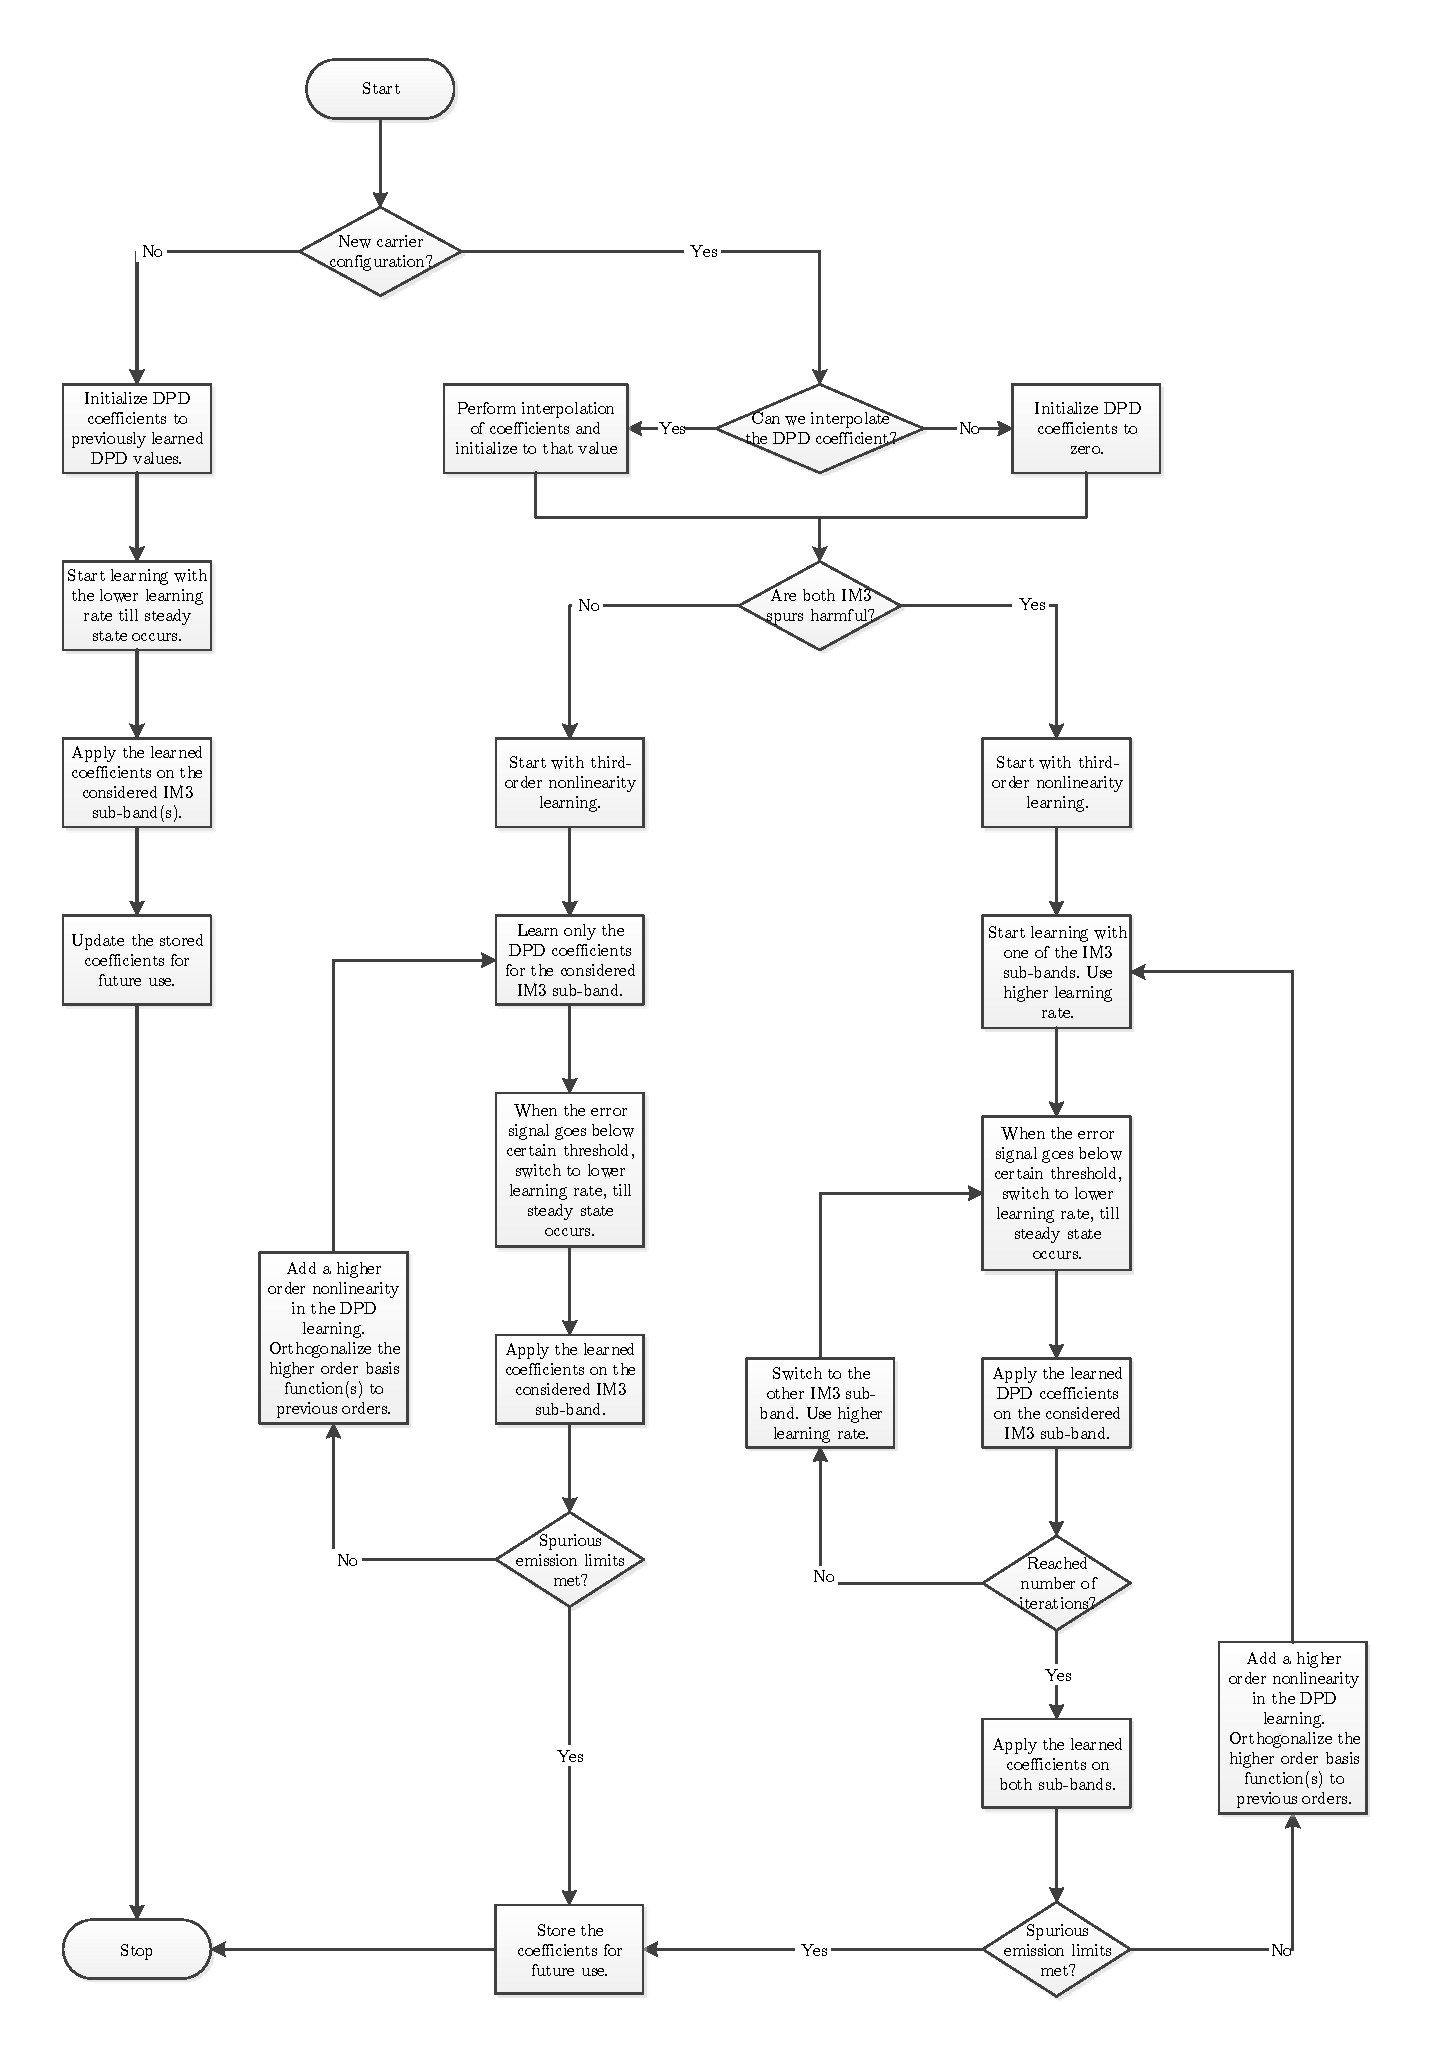
\includegraphics[width=0.89\textwidth]{./Figures/SystemFlowChart.pdf}}
	\caption[]{Flow chart of the proposed iterative sub-band DPD solution.}
	\label{fig:SystemFlowChart}
\end{figure*}
In this section, the overall flow of the proposed DPD processing is summarized and presented, thus putting all the bits and pieces together. 
Fig. \ref{fig:SystemFlowChart} presents a flow chart illustrating the overall DPD system processing including the iterative IM3$\pm$ learning, sequential learning for the higher nonlinearity orders, as well as the convergence speed improvement proposals. 
In case both IM3 sub-bands are required to be suppressed, an iterative IM3$\pm$ third-order sub-band DPD learning step is performed after which the spurious emissions are checked to see whether they already meet the emission requirements or not. 
If they do not satisfy emission requirements, an additional nonlinearity order is added with iterative IM3$\pm$ learning, and so on. 
In all the learning phases, the DPD learning rate $\mu$ is varied according to the residual correlation between the observed IMD emissions and the corresponding basis function(s), in order to improve the learning speed, as explained in Algorithm \ref{alg:mu}. 
Also whenever the DPD coefficients converge, they can be stored in the memory as starting points when the transmission scenarios are repeated. 
In the next section, comprehensive experimental results are presented using the \textsc{Warp}Lab setup demonstrating the effectiveness of the proposed DPD solution.

\import{./}{Section_WarpLabResults.tex}

\section{Conclusion}
In this paper an iterative IM3 sub-band DPD learning algorithm has been proposed. 
A sequential learning procedure where higher nonlinearity orders were added one at a time was also presented in order to reduce the complexity and flexibility of the DPD. 
Additionally, the convergence speed of the proposed DPD has been improved by two methods, while not sacrificing the DPD performance. 
The first used a variable learning rate which switches from high speed to lower speed once the loop becomes close to convergence. 
The second method starts the DPD learning from previously learned points to reduce convergence time. 
A \textsc{Warp}Lab implementation of the proposed DPD solution has been demonstrated showing excellent performance with up to 20 dB suppression in the undesired spurious emissions.

%\begin{acknowledgements}
%If you'd like to thank anyone, place your comments here
%and remove the percent signs.
%\end{acknowledgements}

% BibTeX users please use one of
%\bibliographystyle{spbasic}      % basic style, author-year citations
%\bibliographystyle{spmpsci}      % mathematics and physical sciences
%\bibliographystyle{spphys}       % APS-like style for physics
\bibliographystyle{ieeetr} 
\bibliography{Ref}   % name your BibTeX data base

\iffalse %Comment out the template bib and other things I might want to look at

\begin{figure}
% Use the relevant command to insert your figure file.
% For example, with the graphicx package use

\includegraphics{example.eps}
% figure caption is below the figure
\caption{Please write your figure caption here}
\label{fig:1}       % Give a unique label
\end{figure}
%
% For two-column wide figures use
\begin{figure*}
% Use the relevant command to insert your figure file.
% For example, with the graphicx package use

\includegraphics[width=0.75\textwidth]{example.eps}
% figure caption is below the figure
\caption{Please write your figure caption here}
\label{fig:2}       % Give a unique label
\end{figure*}
%
% For tables use
\begin{table}
% table caption is above the table
\caption{Please write your table caption here}
\label{tab:1}       % Give a unique label
% For LaTeX tables use
\begin{tabular}{lll}
\hline\noalign{\smallskip}
first & second & third  \\
\noalign{\smallskip}\hline\noalign{\smallskip}
number & number & number \\
number & number & number \\
\noalign{\smallskip}\hline
\end{tabular}
\end{table}

% Non-BibTeX users please use
\begin{thebibliography}{}
%
% and use \bibitem to create references. Consult the Instructions
% for authors for reference list style.
%
\bibitem{RefJ}
% Format for Journal Reference
Author, Article title, Journal, Volume, page numbers (year)
% Format for books
\bibitem{RefB}
Author, Book title, page numbers. Publisher, place (year)
% etc
\end{thebibliography}
\fi

\end{document}
% end of file template.tex

